\newpage
\appendix

\section{A Learning-based Approach}
\label{sec:heuristic}
  
A drawback of the MILP approach is that the generated models grow with the 
size of the database and query log.
However, we argue that the encoded information is necessary in order to generate a sufficient set of constraints that result in a good repair.
In this section, we examine an alternative, simpler, decision tree-based approach called \dt. 
We show that even in a simple case of a single query log and a complete complaint set, it is expected to perform poorly.
We will first describe how to model the repair process using a decision tree,
and then we will present and discuss experimental results that illustrate its limitations.

\subsection{Modeling Repairs with Decision Trees}

Rule-based learners are used in classification tasks to generate a set of rules, or conjunctive predicates that best classify a group of labeled tuples.
The rules are non-overlapping, and each is associated with a label---a tuple that matches a given rule is assigned the corresponding label.
These rules exhibit a natural parallel with SQL \texttt{WHERE} clauses, 
which can be viewed as labeling selected tuples with a positive label and rejected tuples with a negative label.
Similarly, the structure of the rules is identical to those that \sys is designed to repair.
Thus, given the database tuples labeled to describe the errors, we may use a rule-based learner to
generate the most appropriate \texttt{WHERE} clause.
We focus our attention on rule-based learners;
specifically, we experiment with the C4.5~\cite{quinlan1987} decision tree learner, which is an 
exemplar of rule-based learners.

A core limitation of this classification-based approach is that there is no means to 
repair \texttt{SET} clauses, which modify data values rather than simply label them.
We resolve this with a two step approach.
We first use the decision tree to generate a repair for the
\texttt{WHERE} clause, and then use the modified query to identify repairs for the \texttt{SET} clause.
The need for this two step procedure limits this approach to encoding and repairing at most one query
at a time.

\noindent
\textbf{Repairing the WHERE Clause:}
The \texttt{WHERE} clause of an update query is equivalent to a
rule-based binary classifier that splits tuples into two groups:
(1)~tuples that satisfy the conditions in the \texttt{WHERE} clause
and (2)~tuples that do not. A mistake in a query predicate can 
cause a subset of the tuples to be misclassified, and in turn,
translate into data errors. 
Therefore, repairing the complaints corresponds to repairing the imprecise classification. 

The repair works as follows: For an incorrect query $q$, let
$D_0$ be the database state before $q$, and $D_1^*$ the \emph{correct}
database state that should have been the result after $q$, if $q$ were correct.
We use each tuple $t \in D_0$ as an element in the input training data
for the classifier where the values (of each attribute) of $t$ define
the feature vector and the label for $t$:
	\[
    label(t)= 
    \begin{cases}
    true & \textrm{if\ }D_0.t \neq D_1^*.t\\
    false              & \text{otherwise}
    \end{cases}
\]
The \texttt{true} rules generated by the decision tree trained on this labeled dataset 
forms a disjunction of rules that constitute the repaired \texttt{WHERE} clause.


\noindent
\textbf{Repairing the SET Clause:}
The \texttt{WHERE} clause repair proposed by the classifier may not completely repair 
the complaints if there was also an error in the \texttt{SET} clause. 
In this case, we execute a second repair step.
\begin{figure}[!htb]
\centering
  \begin{subfigure} [t]{.75\columnwidth}
  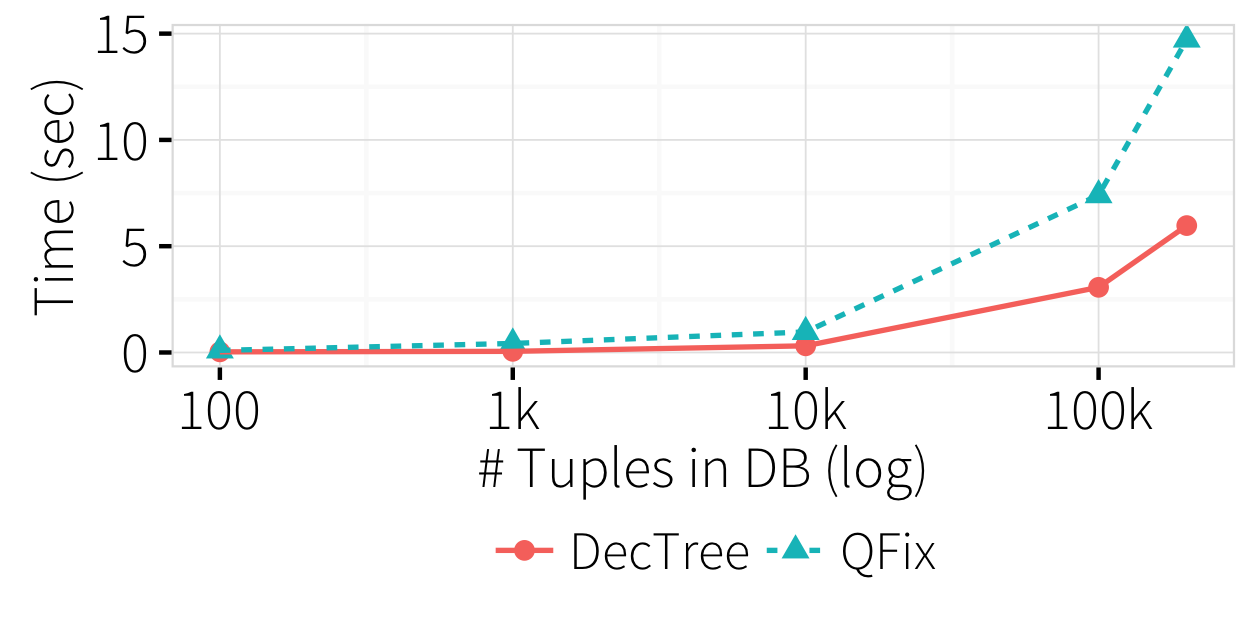
\includegraphics[width = \columnwidth]{figures/heuristictime}
  \caption{Comparison on Performance.}
  \label{f:heuristic_time} 
  \end{subfigure}\\

  \begin{subfigure} [t]{.75\columnwidth}
  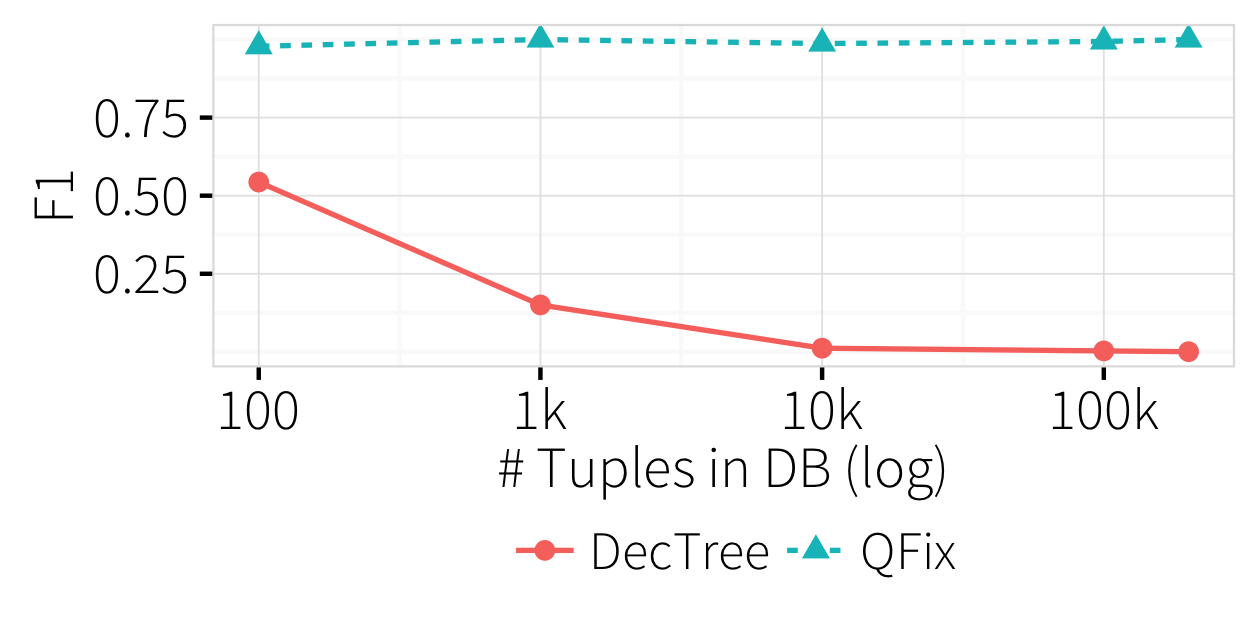
\includegraphics[width = \columnwidth]{figures/heuristicacc}
  \caption{Comparison on Accuracy.}
  \label{f:heuristic_acc} 
  \end{subfigure}
 \caption{\dt compared with \sys}
 \label{f:heuristic}
\end{figure}

We model the errors as a simple linear system of equations: 
each expression in the \texttt{SET} clause is translated into a
linear equation in the same fashion as described in Section~\ref{sec:sol}.
Directly solving the system of equations for the undetermined variables 
will generate the desired repair for the \texttt{SET} expression.



\subsection{Experimental Results}

To illustrate these shortcomings, we compare \dt with \sys using a simplified version of the setup from Section~\ref{sec:experiments} that favors \dt.
We restrict the query log to contain a single query that is corrupted, use a complete complaint set  and vary the database size.
We use the following query template, where all \texttt{SET} clauses assign the attributes to constants,
and the \texttt{WHERE} clauses consist of range predicates:

{\scriptsize
\begin{verbatim}
  UPDATE table
  SET  (a_i=?), ...
  WHERE a_j in [?,?+r] AND ...
\end{verbatim}
}

Figure~\ref{f:heuristic_time} shows that although the runtime performance of \dt is better than \sys by small a constant factor ($\sim 2.5 \times$),
both runtimes degrade exponentially.
In addition, the \dt repairs are effectively unusable as their accuracy is low: the F1-score starts at $0.5$ and rapidly degrades towards $0$.
From these empirical results, we find that \dt generates low-quality repairs even under the simplest conditions---an approach
that applies \dt over more queries is expected to have little hope of succeeding.



There are three important reasons why \dt, and any approach that focuses on a single query at a 
time\footnote{Although our incremental approach tries to generate a repair for a single
query at a time, it encodes all subsequent queries in the log.}, will not perform well.
  \begin{figure*}[t]
  \centering
      \begin{subfigure} [t]{.3\textwidth}
    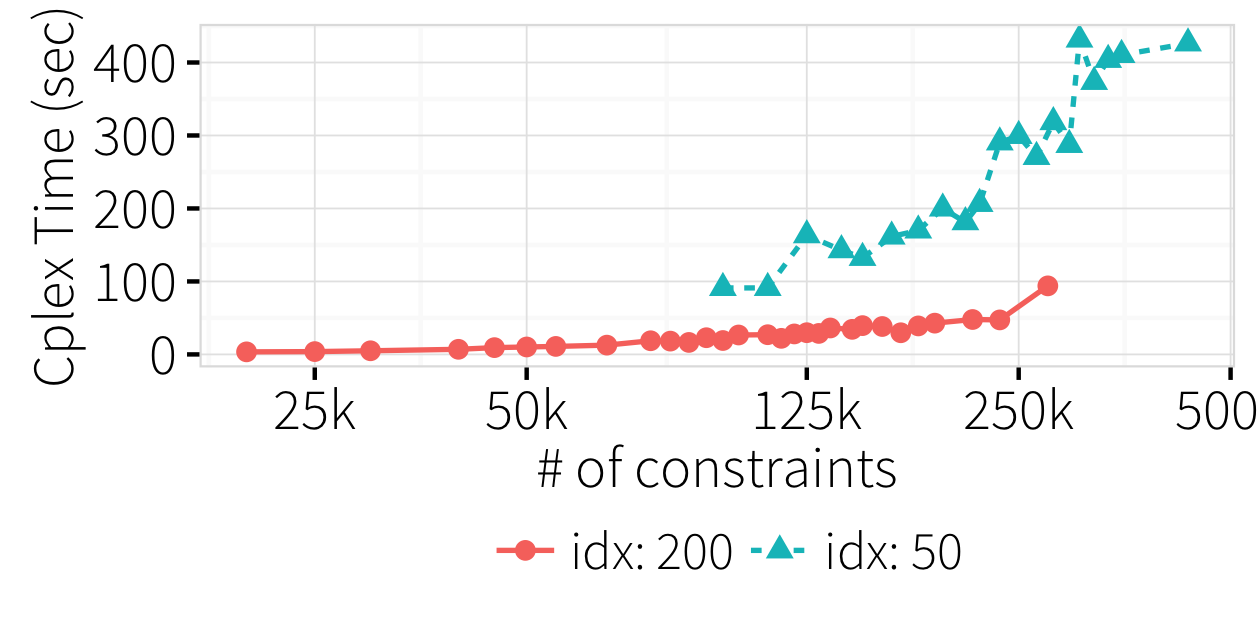
\includegraphics[width = .99\columnwidth]{figures/num_cons_time}
    \vspace*{-.25in}
    \caption{\# of constraints vs. solver solving time.}
    \vspace*{-.1in}
    \label{f:cons_vs_time} 
    \end{subfigure}
    \begin{subfigure} [t]{.3\textwidth}
    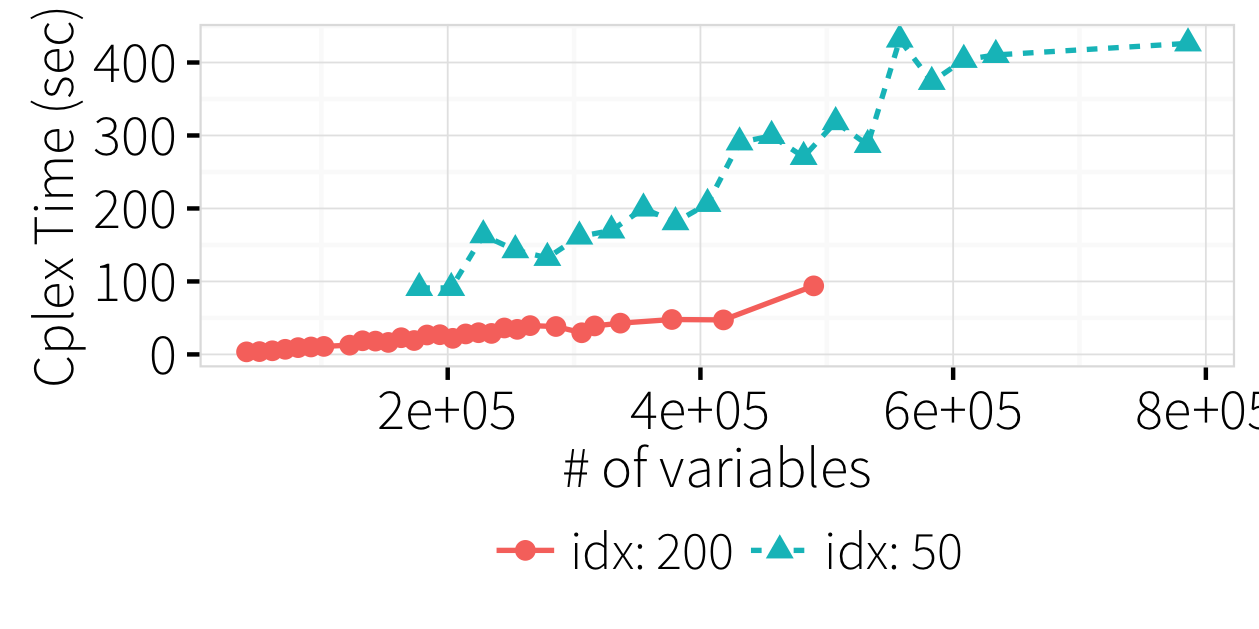
\includegraphics[width = .99\columnwidth]{figures/num_vars_time}
    \vspace*{-.25in}
    \caption{\# of undetermined variables vs. solver solving time.}
    \vspace*{-.1in}
    \label{f:var_vs_time} 
    \end{subfigure}
    \begin{subfigure} [t]{.3\textwidth}
    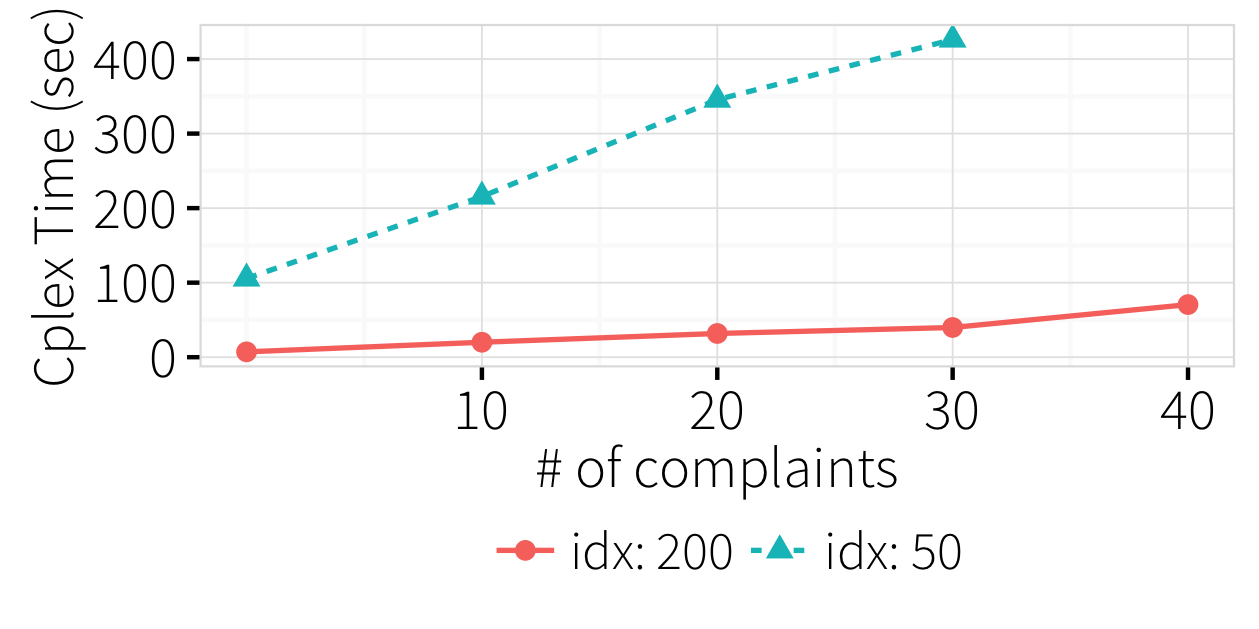
\includegraphics[width = .99\columnwidth]{figures/num_compl_time}
    \vspace*{-.25in}
    \caption{\# of compl. vs. solver solving time.}
    \vspace*{-.1in}
    \label{f:compl_vs_time} 
    \end{subfigure} 
    \iffalse
    \begin{subfigure} [t]{.3\textwidth}
    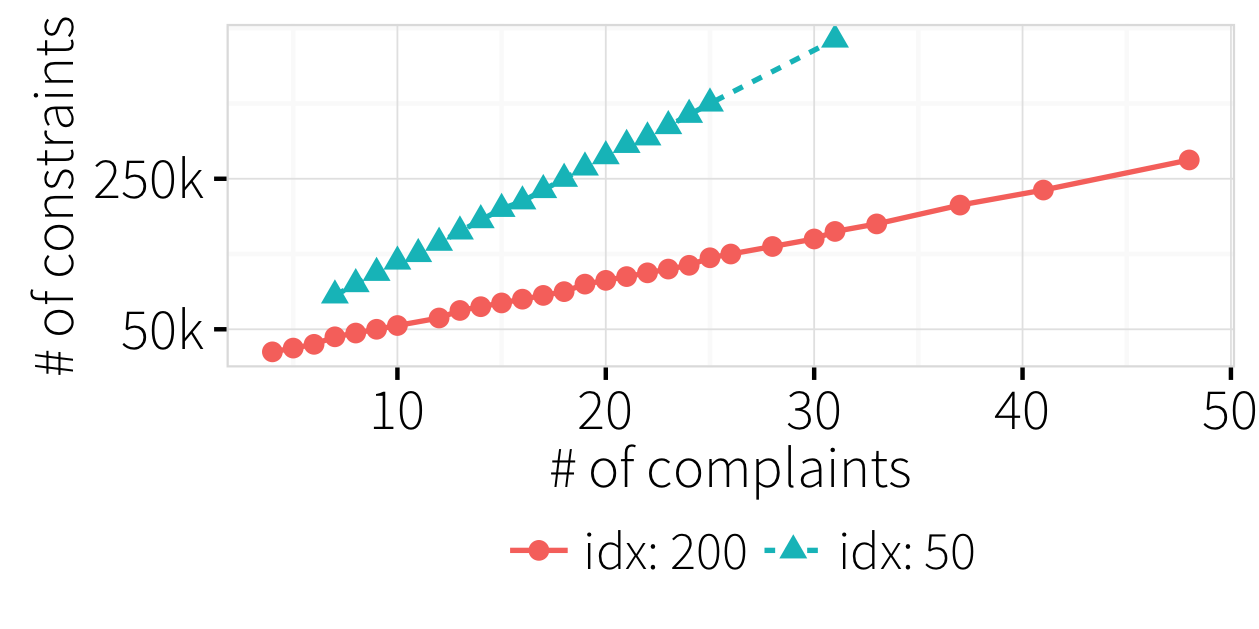
\includegraphics[width = .99\columnwidth]{figures/num_compl_cons}
    \vspace*{-.25in}
    \caption{\# of constraints vs.\# of compl.}
    \vspace*{-.1in}
    \label{f:compl_vs_cons} 
    \end{subfigure}
    \begin{subfigure} [t]{.3\textwidth}
    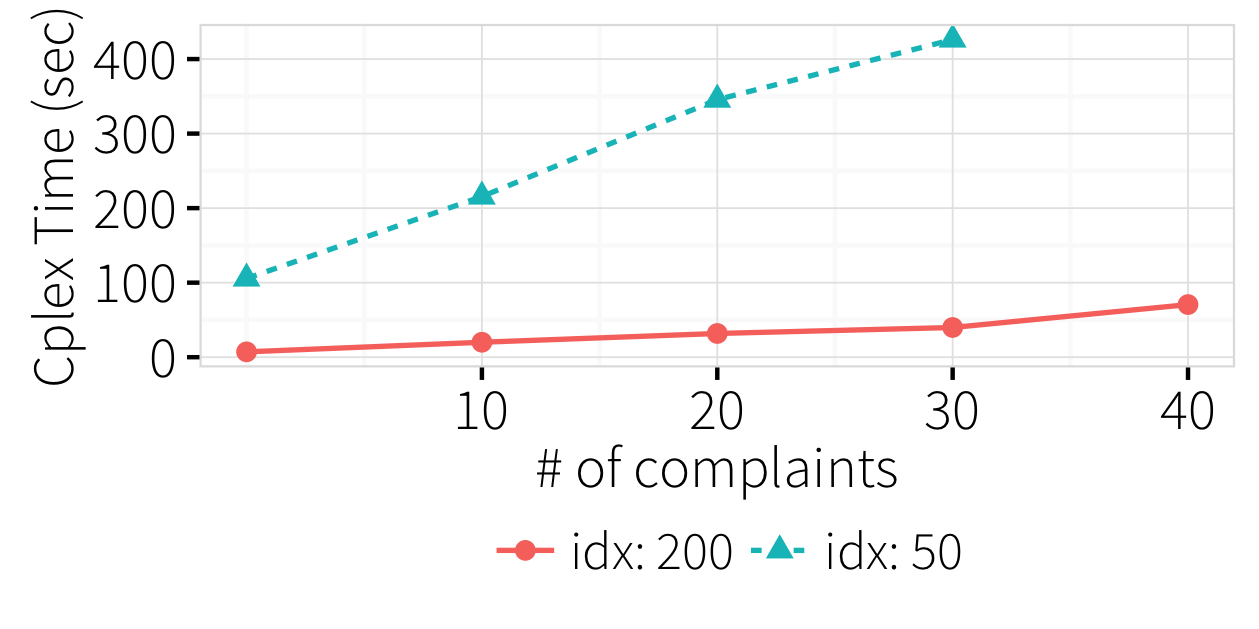
\includegraphics[width = .99\columnwidth]{figures/num_compl_time}
    \vspace*{-.25in}
    \caption{\# of undetermined variables vs. \# of compl.}
    \vspace*{-.1in}
    \label{f:compl_vs_time}
    \end{subfigure}
    \fi
   \caption{Solver solving time grows with all three factors: number of constraints, number of undermined variables and number of complaints. }
   \vspace*{-.1in}
   \label{f:soltime}
  \end{figure*}
\begin{itemize}[itemsep=1pt, leftmargin=5mm]
\item \textbf{Single Query Limitation: }
In principle, one could attempt to apply this technique to the
entire log one query at a time, starting from the most recent query.
Even ignoring the low repair accuracy shown in Figure~\ref{f:heuristic_acc},
this approach is infeasible.
Consider that we generate a labeled training dataset to repair $q_i$ 
using the query's input and output database states $D_{i-1}$ and $D_i^*$.
Note that $D_i^*$ is the theoretically \emph{correct} database state assuming no errors in the query log.
We would need to derive $D_i^*$ by applying the complaint set to $D_n$ to create $D_n^*$, and roll back the database state.
Unfortunately, \texttt{UPDATE} queries are commonly surjective such
that their inverses are ambiguous, which means that it is often
impossible to derive $D_i^*$. In contrast, the incremental version of
\sys can bypass this problem by encoding subsequent queries in the log
in a MILP representation.


\item \textbf{Structurally Different \texttt{WHERE} Clause Results: } 
The basic classifier approach simply learns a set of rules to minimize
classification error, and can derive a clause whose struture is arbitrarily 
different from the original query's \texttt{WHERE} clause.
Although it may be possible to incorporate a distance measure as part of the decision tree
splitting criteria, it is likely to be a heuristic with no guarantees.


\item \textbf{High Selectivity, Low Precision: }
Classifiers try to avoid overfitting by balancing the complexity of the rules with classification accuracy.
This is problematic for highly selective queries (e.g., primary key updates), because the classifier
may simply ignore the single incorrect record and generate a rule such as \texttt{FALSE}.
In fact, this form of severely imbalanced data continues to be a challenge for most major classification algorithms~\cite{he2009learning, galar2012review}. 
Thus, we believe that alternative classification algorithms would not improve on these results. 
Compound with the fact that many workloads are primarily composed of
key update queries~\cite{oltpbench} this issue severely limits the
applicability of learning-based approaches.

\end{itemize}








\section{MILP Solver Performance}
\label{app:solvtime}
\subsection{Factors Relevant to Solver Performance}

\ewu{reference other constraint performance papers}
\xlw{
In this section, we study factors that influence the MILP solver solving time. In this paper, we
use IBM CPLEX~\cite{cplex2014v12} as a black box to solve the constructed MILP problems. Similar to many solver performance studies~\cite{atamturk2005integer, meindl2012analysis, gearhart2013comparison}, 
we majorly study the connection between solver performance between \textit{the number of constraints} and \textit{the number of variables} in the constructed MILP problem. For this, we create \texttt{UPDATE}-only workloads using our synthetic data generator for 300 queries with constant \texttt{SET} clause and range \texttt{WHERE} clause: }

{\scriptsize
\begin{verbatim}
  UPDATE table
  SET  (a_i=?), ...
  WHERE a_j in [?,?+r] AND ...
\end{verbatim}
}
\xlw{We further corrupt two query indexes, $q_{50}$ and $q_{200}$, to create the dirty query logs. }

\smallskip
\emph{Number of Constraints: } \xlw{We first study the relationship between solver performance and number of constraints. From Figure~\ref{f:cons_vs_time}, we observe that solver solving time is roughly positive proportional, with tiny fluctuation, to the number of constraints in both corrupt indexes. This is expected because increasing the number of constraints by large scale usually accompany with significantly greater amount of variables in the MILP problem, which lead to harder MILP problems by natural. However, MILP problems with slightly larger amount of constraints sometimes could be even easier to solve since the additional constraints help pruning the searching space for similar amount of variables.}

\smallskip
\emph{Number of Variables: } \xlw{Similar to the previous experiment, we next compare the solver solving time with the number of variables. As shown in Figure~\ref{f:var_vs_time}, we find highly correlated trends compare to Figure~\ref{f:cons_vs_time}. This is due to the way we construct the MILP problem: the number of constraints and the number of variables grows linearly with the number of queries and the number complaints. 
}


\iffalse
 In our experiments we found that increasing the number of constraints by increasing the database, query log, or complaint set sizes aversely affects the solver performance,
  solver performance has been shown to \emph{improve} as constraints that effectively reduce the problem space are added to the problem.  
  Thus, we now focus on the effects on the number of undetermined variables, which strictly increases the problem space.
  We keep the number of constraints fixed, however increase the number of undetermined variables by \ewu{XL fill in}. \xlw{need to rerun exp to get required numbers. We need to gradually increase the batch size to achieve this. }

\fi

\smallskip
\emph{Takeaway: }\xlw{ In Figure~\ref{f:compl_vs_time} we illustrate the above argument by comparing the average solver solving time between the number of complaints at two different corrupt indexes. As expected, with the same number of complaints, the solver solving time for corrupt index $50$ is significantly higher than index $200$ since the number of queries encoded in each problem is $250$ and $100$ respectively. In contract, with the same corrupt query index, problems with higher amount of complaints has much higher average solver solving cost than problems with lower amount of complaints. }

\subsection{Factors Relevant to the Number of Complaints}
\xlw{
From the above experiments, we observe that the solver solving time is higher correlated to the number of complaints and the number of queries we encoded in a MILP problem. The number of queries can be easily controlled by a particular parameter. The number of complaints, on the other hand, is influence by various factors including the \texttt{SET} clause type, corrupt query index, query skewness, \texttt{WHERE} clause range, and some random factors. To better understand factors that control the size of the complaint set, we ran simulations using a database with $20$ attributes, and a query log of size $1000$ containing
either all constant or relative \texttt{SET} clause \texttt{UPDATE} queries.
We varied the number of corrupt index uniformly throughout the query log, and additionally varied
the skew and range parameters to study how they affect the size of the complaint sets.}
   \begin{figure*}[ht]
  \centering
  \begin{subfigure} [t]{.3\textwidth}
    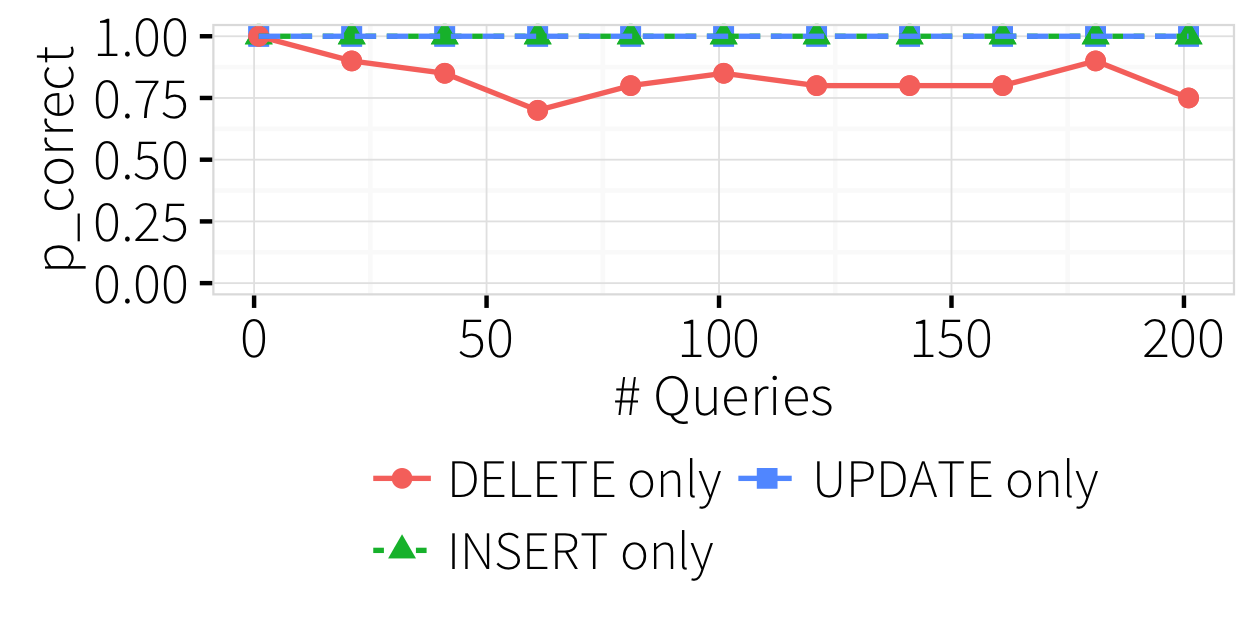
\includegraphics[width = .99\columnwidth]{figures/indelup_acc_idx}
    \vspace*{-.25in}
    \caption{Correct repair ratio vs. query types}
    \label{f:querytyperatio} 
    \end{subfigure}
    \begin{subfigure} [t]{.3\textwidth}
    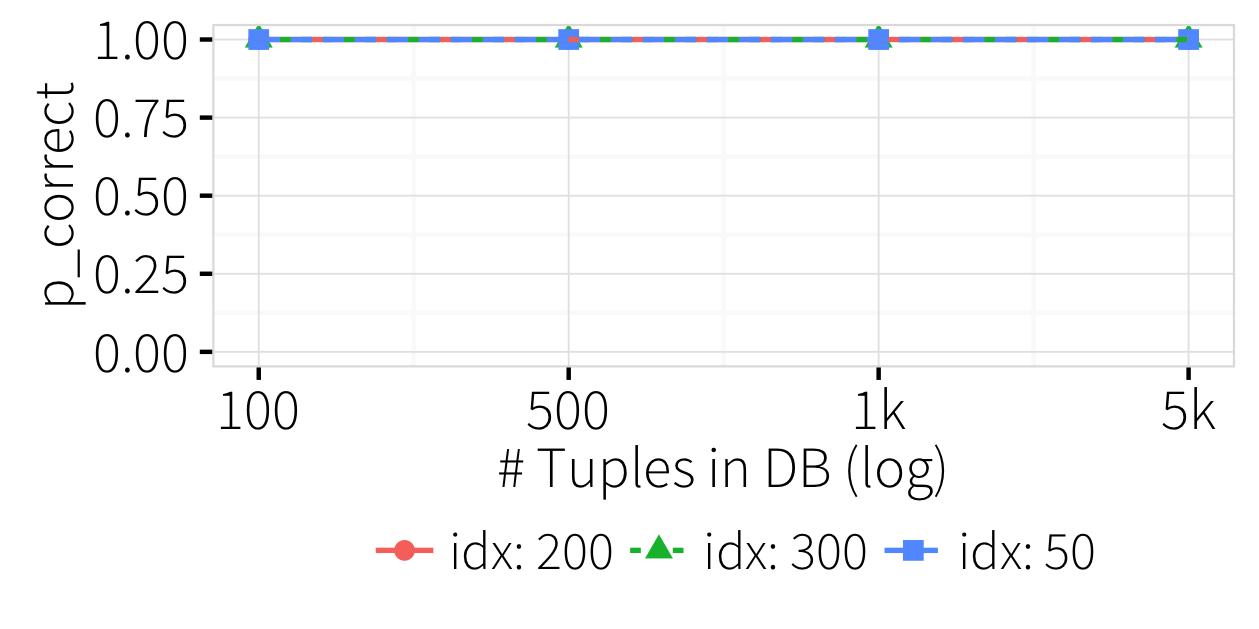
\includegraphics[width = .99\columnwidth]{figures/dbsize_acc_idx}
    \vspace*{-.25in}
    \caption{Correct repair ratio vs. database sizes}
    \label{f:dbsizeratio} 
    \end{subfigure}
    \begin{subfigure} [t]{.3\textwidth}
    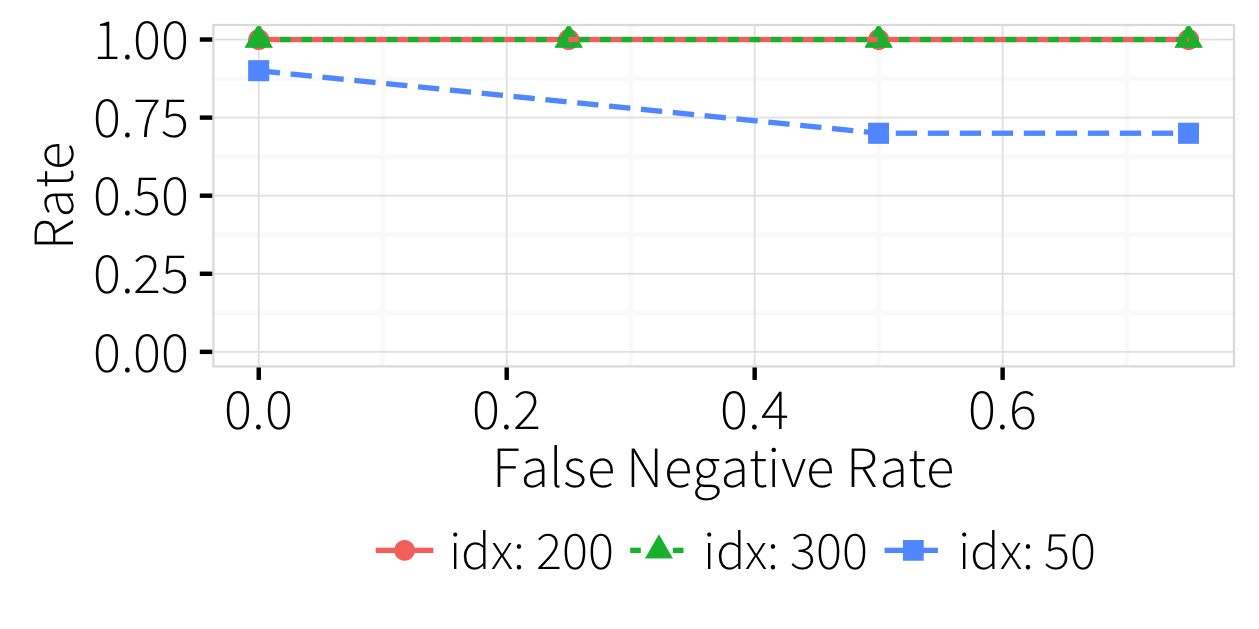
\includegraphics[width = .99\columnwidth]{figures/noise_fn_acc_idx}
    \vspace*{-.25in}
    \caption{Correct repair ratio vs. false negatives}
    \label{f:fnratio} 
    \end{subfigure} \\
    \begin{subfigure} [t]{.3\textwidth}
    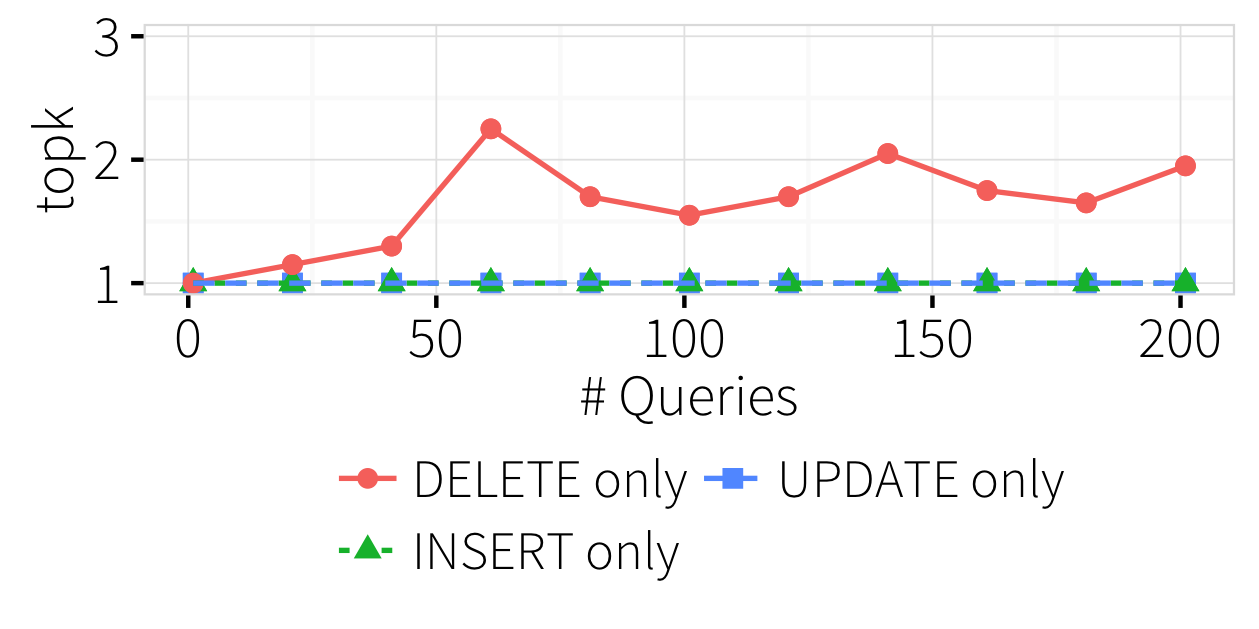
\includegraphics[width = .99\columnwidth]{figures/indelup_fixcount}
    \vspace*{-.25in}
    \caption{Top-k vs. query types. }
    \vspace*{-.1in}
    \label{f:querytypefixcount} 
    \end{subfigure}
    \begin{subfigure} [t]{.3\textwidth}
    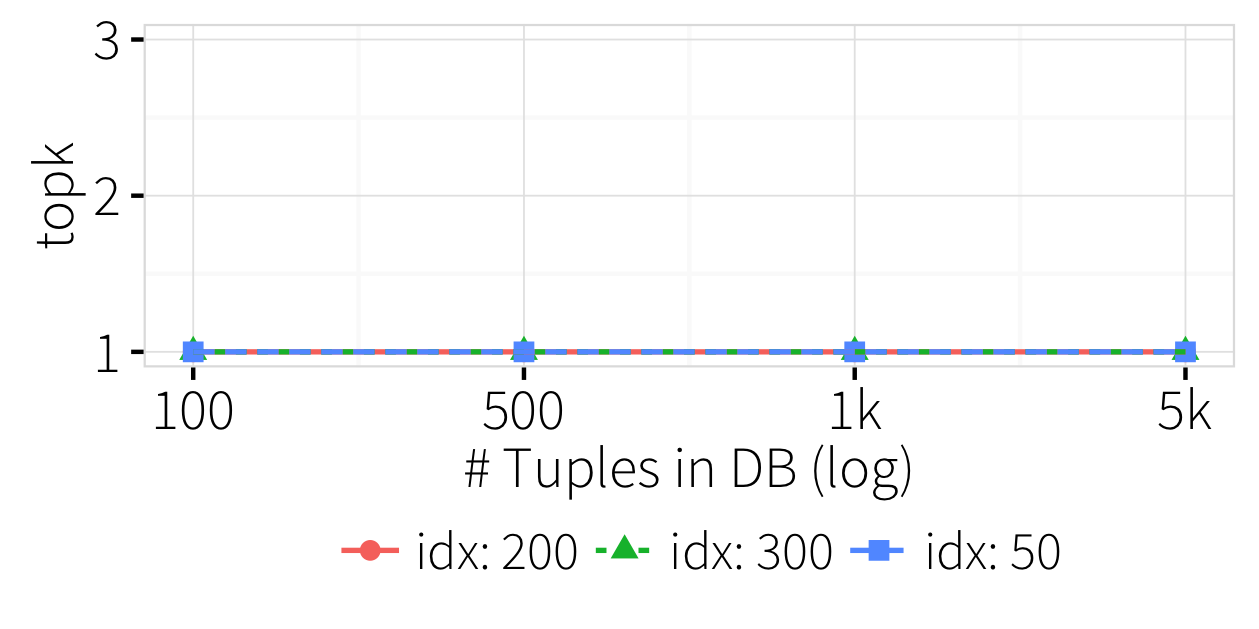
\includegraphics[width = .99\columnwidth]{figures/dbsize_fixcount}
    \vspace*{-.25in}
    \caption{Top-k vs. database sizes. }
    \vspace*{-.1in}
    \label{f:dbsizecount} 
    \end{subfigure}
    \begin{subfigure} [t]{.3\textwidth}
    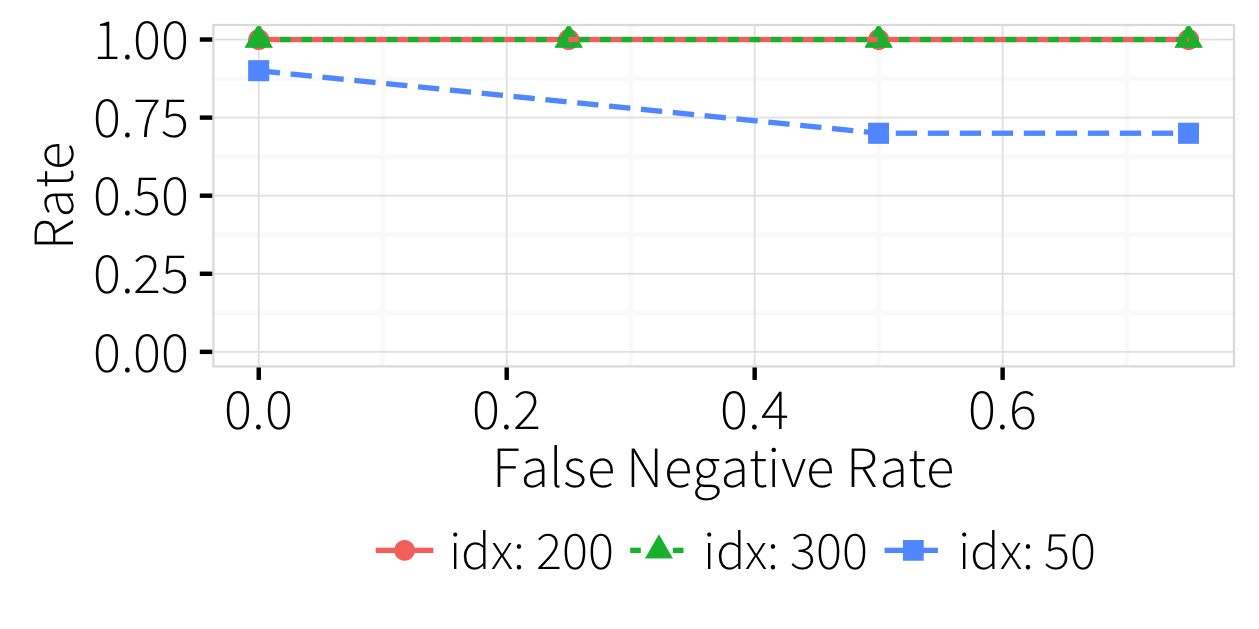
\includegraphics[width = .99\columnwidth]{figures/noise_fn_acc_idx}
    \vspace*{-.25in}
    \caption{Top-k vs. false negatives (\color{red}{not complete!})}
    \vspace*{-.1in}
    \label{f:fnfixcount} 
    \end{subfigure}
   \caption{Correct repair ratio and number of candidate fixes of \sys varies on different types of workloads and false negative rate but remain 
   stable for with increasing number of tuples on \texttt{UPDATE} workload.}
   \vspace*{-.1in}
   \label{fig:truerate}
  \end{figure*}
  \begin{figure}[!h]
  \centering
  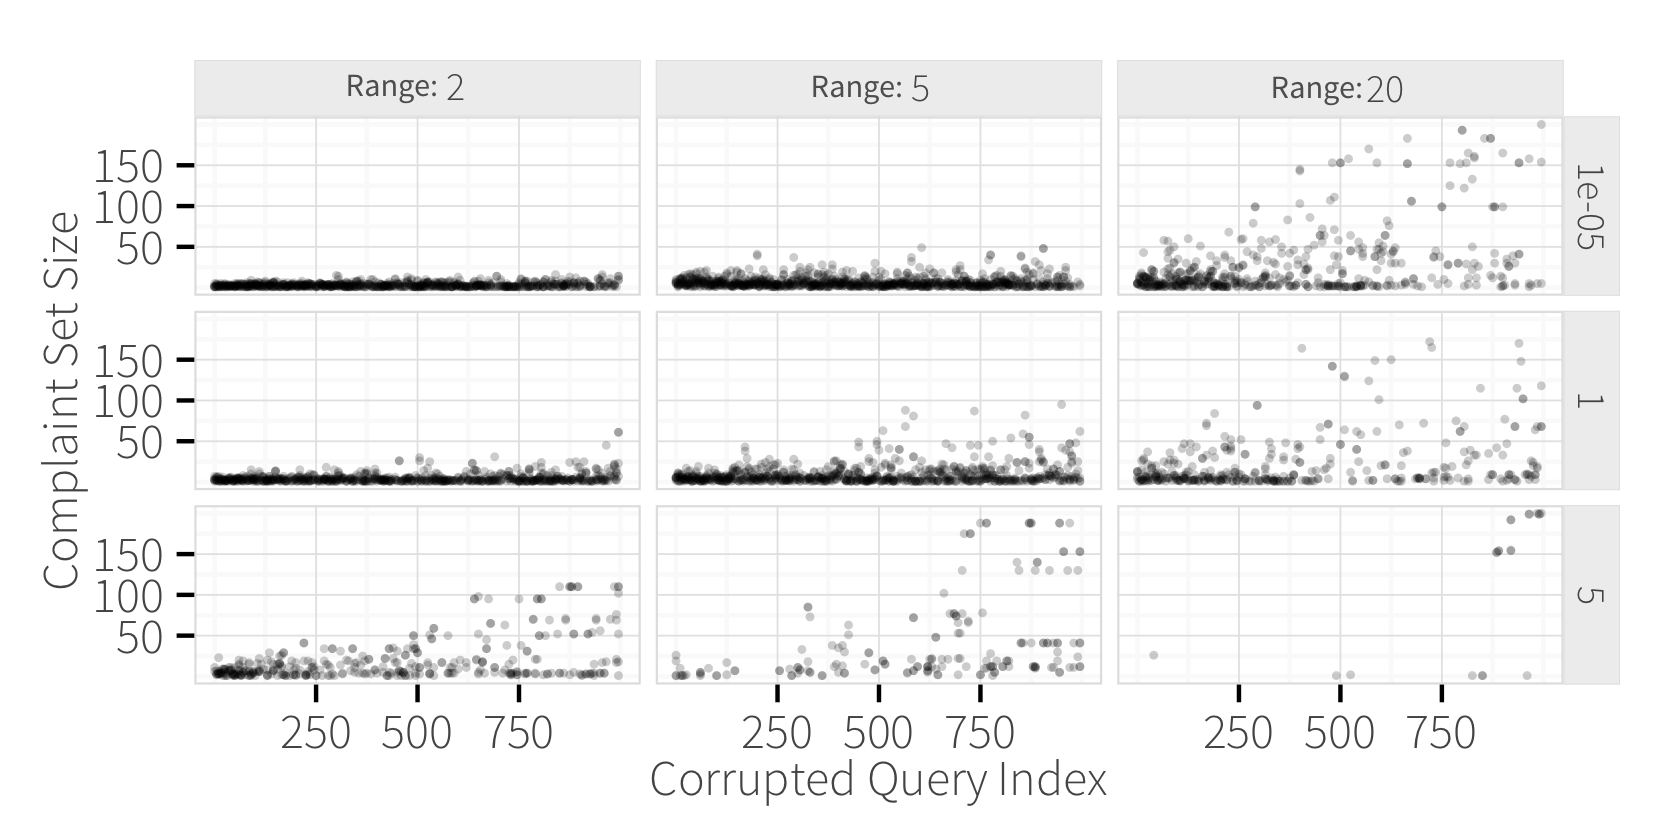
\includegraphics[width = 3in]{figures/qidxsimulation/qidx_v_ncomplaints_20attrs_const}
  \caption{Corrupt query index, skew, range vs complaint set size for \textit{constant} \texttt{SET} clauses.}
  \label{f:qidx_v_ncomplaints_const} 
  \end{figure}
 

\smallskip
\emph{Constant \texttt{SET} clause: } \xlw{Figure~\ref{f:qidx_v_ncomplaints_const} plots a representative set of parameters including corrupt query index, range, and skew. We plot one point
for each corrupted query index that results in a complaint set with at least one complaint. 
These results highlight several interesting trends:  With small update range and small skew factor (left upper corner)
the size of the complaint sets are relatively small, and their frequency is constant across the possible query indices.
However as we increase the range and skew, more recent queries are more likely to result in very large complaint sets (at times the size of the database).   
This effect is a symptom of the fact that queries with higher overlap with each other will set groups of tuples to the same value,
and over time, skew the distribution of tuple values to a small number of possible values. 
Thus, more recent corruptions that affect a large cluster of similar tuples will result in a large complaint set.
And the possibility of query overlap increases with update range and skew as these two factors increase the likelihood that queries share the same \texttt{WHERE} and \texttt{SET} clause. }

\begin{figure}[!h]
\centering
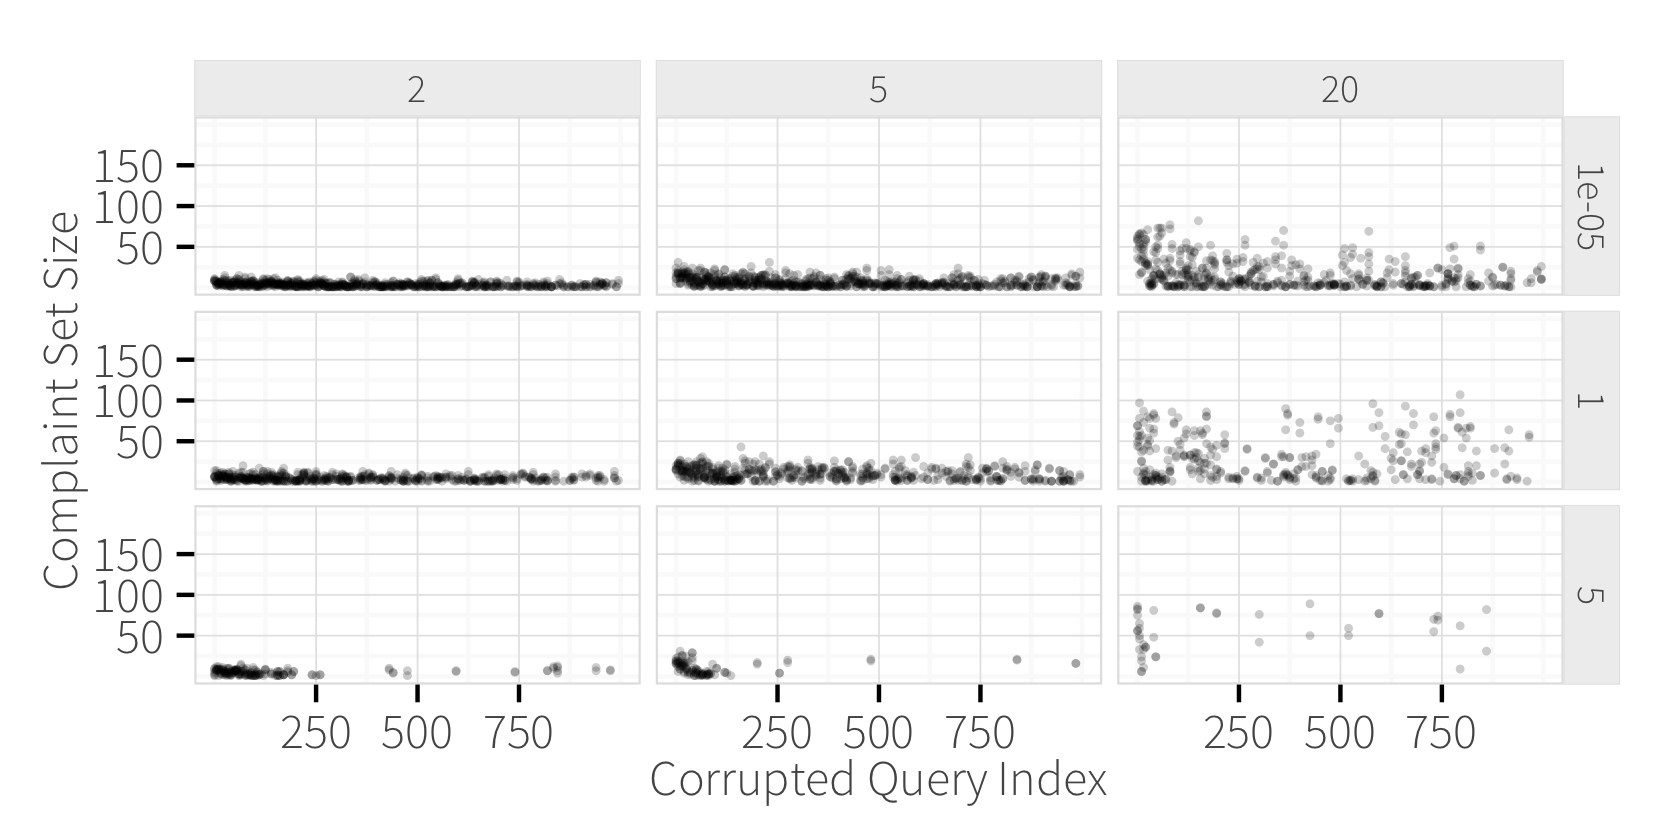
\includegraphics[width = 3in]{figures/qidxsimulation/qidx_v_ncomplaints_20attrs_rel}
\caption{Query index vs complaint set size for $set = rel$.}
\label{f:qidx_v_ncomplaints_rel} 
\end{figure}

\smallskip
\emph{Relative \texttt{SET} clause: } \xlw{In contrast to \textit{constant} \texttt{SET} queries, Figure~\ref{f:qidx_v_ncomplaints_rel} executes the 
same experiment using \textit{relative} \texttt{SET} queries.  In this setting, we find that the trend is
reversed, and older corruptions tend to result in larger complaint sets.  This is because,
subsequent \texttt{UPDATE} queries increment or decrement the attribute value, rather than
overwriting it with a constant value.  The clustering of data values due to query overlap
then increases the number of other tuples affected.
}



\begin{figure*}[ht]
	{\scriptsize
    \begin{minipage}[t]{0.2\textwidth}
         \vspace{0pt} 
         \centering
        \begin{tabular}{lllll}
            \multicolumn{5}{l}{\emph{table}: $D_0$}\\
            \toprule
            \textbf{ID}  & \textbf{$a_1$}    & \textbf{$a_2$} & \textbf{$a_3$} & \textbf{$a_4$} \\
            \midrule
            0 & 8 & 4 & 12 & 28\\
            1 & 2 & 10 & 15 & 3\\
            \bottomrule
            \\
    \end{tabular}
    \end{minipage}
     \begin{minipage}[t]{0.5\textwidth}
         \vspace{0pt} 
         \centering
        \begin{tabular}{l}
            \multicolumn{1}{l}{A \texttt{DELETE} workload  $\mathcal{Q}_{del}$:                                                            }\\
             \toprule
            \texttt{Q1: DELETE FROM table WHERE $a_2$ in \sout{[3,5]} {\color{red}[30, 50]}} \\
   			\texttt{Q2: DELETE FROM table WHERE $a_3$ in [7, 8] }\\ \hline
    \end{tabular}
    \end{minipage}
    \begin{minipage}[t]{0.2\textwidth}
         \vspace{0pt} 
         \centering
       \begin{tabular}{lllll}
            \multicolumn{5}{l}{\emph{table}: $D_1$ after execute $\mathcal{Q}_{del}$}\\
            \toprule
            \textbf{ID}  & \textbf{$a_1$}    & \textbf{$a_2$} & \textbf{$a_3$} & \textbf{$a_4$} \\
            \midrule
            \rowcolor{mid-gray}
            \sout{0} & \sout{8} & \sout{4} & \sout{12} & \sout{28}\\
            1 & 2 & 10 & 15 & 3\\
            \bottomrule
            \\
\end{tabular}
    \end{minipage} \\
  \begin{minipage}[t]{0.2\textwidth}
         \vspace{0pt} 
         \centering
        \begin{tabular}{lllll}
        
            
    \end{tabular}
    \end{minipage}
 \begin{minipage}[t]{0.5\textwidth}
         \vspace{0pt} 
         \centering
        \begin{tabular}{l}
   			\multicolumn{1}{l}{A \texttt{UPDATE} workload $\mathcal{Q}_{up}$:                              }\\
   			 \toprule
            \texttt{Q1: UPDATE table SET $a_1$ = 10 WHERE $a_2$ in \sout{[3,5]} {\color{red}[30, 50]}} \\
   			\texttt{Q2: UPDATE table SET $a_4$ = 7 WHERE $a_3$ in [7, 8] }\\ \hline
            \\
    \end{tabular}
    \end{minipage}     
    \begin{minipage}[t]{0.2\textwidth}
         \vspace{0pt} 
         \centering
\begin{tabular}{lllll}
            \multicolumn{5}{l}{\emph{table}: $D_1'$ after execute $\mathcal{Q}_{up}$}\\
            \toprule
            \textbf{ID}  & \textbf{$a_1$}    & \textbf{$a_2$} & \textbf{$a_3$} & \textbf{$a_4$} \\
            \midrule
            \rowcolor{mid-gray}
            0 & \color{red}{8} & 4 & 12 & 28\\
            1 & 2 & 10 & 15 & 3\\
            \bottomrule
            \\
\end{tabular}
    \end{minipage}
}
    \vspace{-2mm}
    \caption{A initial database state $D_0$ and database states after apply $\mathcal{Q}_{del}$ and $\mathcal{Q}_{up}$ on $D_0$. }
    \label{fig:example2}
\end{figure*}
\section{Repairing the Correct Query}
\label{app:index}

The experimental section (Section~\ref{sec:experiments}) primarily focused on performance and accuracy measures of the repairs, and for space constraints, ignored 
whether the proposed repair was actually the correct query (it is possible we fix an incorrect query in a way that resolves the complaint set).
Although we found in most circumstances we identify the correct query to fix, we now turn our attention to better understand 
the conditions when we may fix the incorrect query. 


\subsection{Experimental Results}
To evaluate \sys's ability in identifying the correct query to fix, we use two evaluation metrics to summarize our results over 20 runs.
The first $p_{correct}$ computes the ratio between the number of runs where \sys correctly repairs the corrupt query and where \sys
repairs the wrong query.  The second metric $topk$ measures the number of repairs that \sys proposes before repairing the true corrupt query.
This metric is useful to quantify the extent that \sys's repairs are false positives (though they may correctly resolve the complaint set).
A smaller $topk$ value suggests that \sys is still effective at providing repair \emph{recommendations} as part of a diagnostic interface.

\textbf{Correct repair ratio vs. query types: } In Figure~\ref{f:querytyperatio}, we first evaluate $p_{correct}$ rate on three types of workloads: \sys identifies the correct query to fix ($p_{correct} = 1.0$ and $topk = 1$) for \texttt{UPDATE} and \texttt{INSERT} workloads but unstable and much lower rate for \texttt{DELETE} workload. This is expected since more information of the actual incorrectness get maintained through \texttt{UPDATE} queries by the updated tuple values. However, such information get lost and obscured for \texttt{DELETE} queries as those deleted tuples no longer exist in the database. As a result, actual incorrect queries in \texttt{UPDATE} workloads are much easier to identify than those in \texttt{DELETE} workloads. \texttt{INSERT} workloads are easy to fix by natural since each \texttt{INSERT} query only touches one tuple. 

To further illustrate this, we present the following example of two simple query logs, one for \texttt{DELETE} workload and one for \texttt{UPDATE} workload, that operate on the same initial database state and with the exact same \texttt{WHERE} clauses. 

In the above example, we find that there exist two candidate fixes for the \texttt{DELETE} workload $\mathcal{Q}_{del}$: one can either modify the \texttt{WHERE} clause of $Q2$ to $[12, 12]$ or the \texttt{WHERE} clause of $Q1$ to $[4, 4]$. In addition, the two candidate fixes achieve the exact same final database state. However, there only exists one candidate fix for the \texttt{UPDATE} workload $\mathcal{Q}_{up}$ since values in every attribute must satisfy with the desired database state. According to the converted constraints, modifying $Q2$ cannot solve the problem since it would not fix the value in the incorrect attribute $a_1$.  

\textbf{Top-k vs. query types: } In Figure~\ref{f:querytypefixcount}, we observe the same trend: the $topk$ count for \texttt{UPDATE} and \texttt{INSERT} workloads remain $1$ across all query indexes while the $topk$ count shows unstable and much higher value for \texttt{DELETE} workloads. 


\textbf{Correct repair ratio \& top-k vs. database sizes: } We next narrow down to \texttt{UPDATE} workload and evaluate \sys's behavior with increasing amount of tuples in the database. We observe $p_{correct} = 1$ and $topk = 1$ on different corrupt indexes in all database sizes (Figure~\ref{f:dbsizeratio}~\ref{f:dbsizecount}). 

\textbf{Correct repair ratio \& top-k vs. false negatives: } We finally evaluate \sys on \texttt{UPDATE} workload with increasing false negative rates. Similar to the quality drop in Figure~\ref{f:falsenegative_acc}, we observe the $p_{correct}$ (Figure~\ref{f:fnratio}) rate also suffers from less submitted complaints when errors happen early in the query log. However, \sys achieves above $0.75$ $p_{correct}$ rate for more recent errors (corrupt index is 300 and 200) even with high false negative rate. The $topk$ behaves similar to $p_{correct}$ in which $topk$ increasing with the false negative rate (Figure~\ref{f:fnfixcount}).  